\section{Introduction}
\label{sec:intro}

Histopathology provides a direct view of tissue morphology and is increasingly used to predict clinically meaningful outcomes. Computational pathology now includes models trained directly from whole-slide images (WSIs), often using only a slide-level diagnosis. Such models have been applied to cancer detection and subtyping, weakly supervised slide classification, and prediction of molecular biomarkers from H\&E tissue~\cite{campanella2019clinical,lu2021clam,kather2019msi,shmatko2022ai}. Large pretrained pathology encoders have widened the set of tasks that can be studied with limited labels. CTransPath uses contrastive pretraining; UNI and Virchow learn visual representations from large slide collections; CONCH pairs pathology images with text; and Prov-GigaPath incorporates long-range WSI context~\cite{wang2022ctranspath,chen2024uni,lu2024conch,vorontsov2024virchow,xu2024gigapath}. Strong benchmark performance, however, does not establish how reliably these representations generalize across image sets or feature variations. The evidence used by these models is still difficult to interpret.

The appearance of an H\&E image reflects both the underlying tissue and how the slide was prepared and digitized. Features such as nuclear shape, cell density, and tumor--immune organization can also be linked to staining intensity or to the hospital or laboratory where a slide was prepared. Howard \etal{} showed that standard normalization and augmentation do not fully remove clues about where a slide came from~\cite{howard2021sitespecific}. A model can therefore perform well on a held-out set partly by using clues from how the slides were prepared or scanned. This is one reason post-hoc explanations in medical AI require careful validation~\cite{ghassemi2021falsehope,klauschen2024xai}.

Saliency and attention maps provide spatial localization, but it is often unclear what features within a highlighted region influence the model's prediction. A tumor region may be influential because of nuclear size, immune density, spatial mixing, stain, or a scanner artifact. Adebayo \etal{} also showed that some saliency maps remain visually similar after randomizing model parameters or training labels~\cite{adebayo2018sanity}. In a pathology image, knowing where the model focuses does not reveal which tissue feature influenced its response.

Visual counterfactuals give a more direct test by modifying the input and measuring the resulting prediction. Goyal \etal{} retrieve discriminative changes relative to a target class~\cite{goyal2019counterfactual}. DVCE, DiME, and DiG-IN use diffusion priors to produce realistic classifier-guided edits~\cite{augustin2022dvce,jeanneret2022dime,augustin2024digin}. Pathology studies have used changes between classes to reveal tissue patterns linked to molecular labels~\cite{dolezal2023synthetic}. MoPaDi couples a diffusion autoencoder to a task-specific classifier or multiple-instance model to generate morphological counterfactuals optimized toward a target prediction~\cite{zigutyte2026mopadi}. Several correlated attributes may change during this optimization, making it difficult to attribute the model response to one requested factor.

\begin{figure}[!t]
    \centering
    \vspace{2mm}
    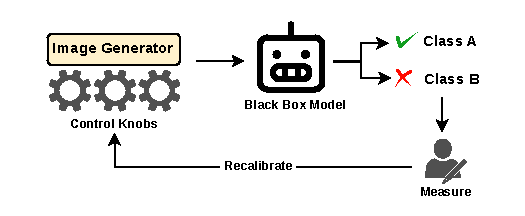
\includegraphics[width=\columnwidth]{../Figure1.pdf}
    \vspace{-6mm}
    \caption{Counterfactual probing with matched, single-control interventions.}
    \label{fig:probing_cartoon}
\end{figure}

\method{} instead starts from a requested intervention rather than a target prediction (Fig.~\ref{fig:probing_cartoon}). We trained \method{} as a diffusion model for controllable H\&E synthesis across cellular spatial organization, nuclear morphology, and stain appearance. It generates matched counterfactuals intended to change one requested factor while preserving the others, and each requested change is verified in the output before downstream use.

We evaluate image realism and whether the generated images reflect the requested interventions before using them for downstream analysis. Candidate selection uses \cellvit{}, while \hovernet{} and \stardist{} provide independent measurements~\cite{horst2026cellvitpp,graham2019hovernet,schmidt2018stardist}. The diffusion model was trained on 1.4 million $512\!\times\!512$ H\&E tiles sampled from 1,114 whole-slide images, with one patient per WSI. The resulting counterfactual datasets are used to probe pathology classifiers, frozen foundation encoders with trained task-specific heads, and survival models.

The paper makes three technical contributions:
\begin{itemize}
    \item a trained diffusion model for controllable H\&E synthesis that reflects requested spatial, morphological, and appearance interventions;
    \item counterfactual datasets spanning these interventions, with generation-side fidelity checks before downstream use; and
    \item an analysis of pathology foundation models and task-specific predictors using the verified counterfactuals to measure their responses to controlled feature changes.
\end{itemize}
